\chapter{Methodology}
\emergencystretch=3em
% Defensive fallbacks in case packages are omitted in root preamble
\providecommand{\mathbb}[1]{\mathbf{#1}}
\providecommand{\varnothing}{\emptyset}
\providecommand{\operatorname}[1]{\mathrm{#1}}
\providecommand{\text}[1]{\mbox{#1}}

\section{Tools and Techniques}

The research and engineering design of the proposed platform is established upon a decoupled, multimodal, and agentic architecture. The framework integrates computer vision for botanical taxon identification, dense vector indexing, labeled property graph modeling, and a hierarchical multi-agent orchestration runtime powered by local Large Language Models (LLMs). The platform operates within a strictly defined academic and demonstration scope focused on 40 clinically and traditionally significant Indian medicinal plant species. 

Incoming user interactions may originate either as botanical leaf photographs or as natural language inquiries regarding medicinal properties, vernacular aliases, plant constituents, or pharmacological mechanisms. The computational framework processes these inputs through a multi-tiered pipeline: visual inputs are evaluated via a fine-tuned deep convolutional neural network and vector similarity engine, natural-language entity references are resolved through a cascaded hybrid search index, and domain knowledge is retrieved from an allow-listed, parameterized Neo4j knowledge graph. High-level planning, retrieval delegation, and answer synthesis are orchestrated by a DeepAgents coordinator operating in conjunction with an outer LangGraph state graph. The principal architectural components and enabling technologies are described below.

\subsection{Next.js and Client-Side Presentation Tier}

The user-facing presentation tier is built with Next.js 15, React 19, and TypeScript, providing a responsive interface for discovery and conversation. Direct cross-origin exposure is eliminated by proxying browser requests through a server-side route at \texttt{/\allowbreak app/\allowbreak api/\allowbreak v1/\allowbreak [...path]/\allowbreak route.ts}.

The frontend architecture is organized into dedicated functional modules:
\begin{itemize}
    \item \textbf{Discovery Interface (\texttt{Discovery.tsx}):} Facilitates taxon identification by providing interactive lexical autocomplete and candidate plant cards displaying botanical names, vernacular aliases, and identification confidence scores.
    \item \textbf{Image Ingestion (\texttt{Upload.tsx}):} Enables drag-and-drop and standard file selection for leaf imagery, handling client-side image validation, dimension checking, and preview generation.
    \item \textbf{Clarification Dialogue (\texttt{Clarification.tsx}):} Renders structured disambiguation prompts when visual or textual classification produces ambiguous candidate sets, allowing users to select an intended botanical identity or submit a higher-quality leaf photograph.
    \item \textbf{Conversation Transcript (\texttt{Conversation.tsx}):} Renders the persistent dialogue stream, supporting streaming Markdown rendering, citation badges, and active session status indicators.
    \item \textbf{Evidence Drawer (\texttt{Evidence.tsx}):} Provides an auditable provenance panel that renders the exact graph traversal paths, node attributes, source literature references, and external identifiers (e.g., PubMed, ChEMBL, and IUCN URLs) associated with any cited fact.
    \item \textbf{Agent Routing Trace (\texttt{AgentRoutingTrace.tsx}):} Exposes real-time agent execution telemetry, visualizing subagent delegation, tool invocations, and graph transitions.
\end{itemize}

Client-to-server communication relies on asynchronous HTTP POST requests for operation dispatch and Server-Sent Events (SSE) for real-time, replayable streaming of model tokens, agent status transitions, and citation metadata.

\subsection{FastAPI Backend and Asynchronous Run Lifecycle}

The core application backend is developed using the FastAPI framework running on Python 3.12 with the Uvicorn ASGI web server. The backend serves as the composition root, managing dependency lifecycles, database connection pools, cross-origin resource sharing (CORS) policies, and API routing. All external and internal data structures are strictly validated using Pydantic v2 schemas defined under \texttt{backend/\allowbreak api/\allowbreak schemas/\allowbreak } and \texttt{backend/\allowbreak contracts/\allowbreak }.

To ensure deterministic single-node execution and prevent concurrent write corruption in local database deployments, application startup establishes a PostgreSQL advisory lease. The operational turn lifecycle is governed by the \texttt{RunManager} service (\texttt{backend/\allowbreak services/\allowbreak runs.py}). To avoid blocking synchronous LLM inferences on the HTTP loop, the backend accepts turns idempotently via SHA-256 request hashing. The service persists an accepted run in PostgreSQL, returns an HTTP 202 Accepted status with a \texttt{RunView} contract, and delegates work to a background task that streams fine-grained operational events (\texttt{run\_started}, \texttt{agent\_started}, \texttt{response\_delta}, \texttt{response\_completed}) over SSE.

\subsection{DeepAgents Multi-Agent Orchestration and Outer LangGraph State Graph}

The orchestration architecture of the platform follows a two-tiered design: an outer checkpointed state graph implemented via LangGraph and an inner hierarchical multi-agent coordinator built on the DeepAgents framework (\texttt{backend/\allowbreak orchestrator/\allowbreak deepagents/\allowbreak runtime.py}).

The outer LangGraph state machine (\texttt{backend/\allowbreak orchestrator/\allowbreak deepagents/\allowbreak graph.py}) encapsulates the entire turn lifecycle. It manages session resumption, error handling, and human-in-the-loop disambiguation. The graph contains two primary execution nodes:
\begin{enumerate}
    \item \texttt{deep\_orchestrator}: Invokes the DeepAgents runtime to plan, delegate, and synthesize answers.
    \item \texttt{clarification}: Engaged when entity discovery is ambiguous or input imagery lacks sufficient botanical detail. This node triggers an interruption operation (\texttt{langgraph.\allowbreak types.\allowbreak interrupt}), yielding execution to the user while serializing the full execution state to PostgreSQL via \texttt{AsyncPostgresSaver}. Upon user input submission, the turn resumes along the identical checkpoint lineage without restarting the dialogue task.
\end{enumerate}

Within the \texttt{deep\_orchestrator} node, a DeepAgents main orchestrator coordinates exactly three compiled specialist subagents:
\begin{itemize}
    \item \textbf{Text/Entity Specialist (\texttt{text\_entity}):} Encapsulates botanical catalog resolution and entity search over PostgreSQL and Qdrant vector indices via the \texttt{resolve\_plant\_names} tool.
    \item \textbf{Image Understanding Specialist (\texttt{image\_understanding}):} Executes leaf image classification and feature-vector nearest-neighbor search via the \texttt{inspect\_uploaded\_image} tool.
    \item \textbf{Knowledge Graph Specialist (\texttt{knowledge\_graph}):} Conducts plant-scoped, parameterized graph traversals over the Neo4j database via the \texttt{retrieve\_plant\_graph} tool.
\end{itemize}

The main orchestrator assesses user queries, formulates delegation plans, enforces query budgets (capped at 3 graph operations per turn), and performs answer repair.

\subsection{Local Large Language Model Integration via Ollama}

Language generation and agent planning are executed locally via Ollama, eliminating external API dependencies. The default model is \texttt{qwen2.5:7b-instruct-q4\_K\_M}, optimized for instruction adherence and structured JSON generation, with \texttt{llama3.1:8b-instruct-q4\_K\_M} supported as an alternative.

Deterministic agent behavior is enforced through specialized system prompts:
\begin{itemize}
    \item \texttt{MAIN\_AGENT\_PROMPT}: Instructs the coordinator to establish a single locked botanical identity before exploring records, delegate factual inquiries to specialist tools, ground all species-specific statements in retrieved graph facts, and distinguish traditional associations from verified clinical efficacy.
    \item \texttt{GRAPH\_AGENT\_PROMPT}: Constrains graph queries to strictly typed, allow-listed retrieval routines and prevents hallucinated citations or raw query formulation.
    \item \texttt{REPAIR\_AGENT\_PROMPT}: Guides post-generation revision when initial drafts contain unfinished procedural plans, unsupported clinical extrapolations, or ungrounded assertions.
\end{itemize}

\subsection{Convolutional Neural Network and Leaf Image Classification}

Visual plant identification utilizes a deep CNN based on the Xception architecture, fine-tuned on medicinal leaf photographs. Processing preprocessed RGB tensors of dimension $300 \times 400 \times 3$, depthwise separable convolutions extract multi-scale spatial features, mapping visual representations into 40-dimensional Softmax class probabilities. Concurrently, Global Average Pooling yields a 2,048-dimensional continuous feature embedding for vector similarity search.

\subsection{Dense Text Embeddings and FastEmbed ONNX Runtime}

To capture semantic relationships across queries, vernacular aliases, and botanical descriptions, dense text embeddings are generated using FastEmbed. FastEmbed executes the \texttt{BAAI/bge-small-en-v1.5} model via the ONNX Runtime, producing 384-dimensional normalized vector representations entirely on local CPU threads.

\subsection{Qdrant Vector Database}

Approximate Nearest Neighbor (ANN) search across dense text and visual vectors is supported by the Qdrant database engine, provisioning two separate vector collections:
\begin{itemize}
    \item \texttt{plant\_names\_v1}: Contains 384-dimensional dense embeddings of all canonical plant names and documented vernacular aliases. Each vector point is indexed alongside structured metadata payloads, including \texttt{generation}, \texttt{plant\_id}, \texttt{language}, and \texttt{alias\_type}.
    \item \texttt{plant\_images\_v1}: Houses 2,048-dimensional $L_2$-normalized feature vectors extracted from 2,507 botanical reference leaf images. Points are indexed with keyword payload indices on \texttt{model\_id}, \texttt{dataset\_id}, and \texttt{label}.
\end{itemize}
Both collections employ cosine distance metrics and Hierarchical Navigable Small World (HNSW) indexing graphs to deliver sub-millisecond nearest-neighbor search.

\subsection{Neo4j Labeled Property Graph Database}

Domain knowledge regarding taxonomy, phytochemicals, biological activities, macromolecular targets, and therapeutic applications is modeled in a Neo4j 5 graph database. The schema enforces integrity across 8 node labels (\texttt{PlantDetails}, \texttt{PlantAlias}, \texttt{PlantPart}, \texttt{Phytochemicals}, \texttt{TherapeuticUse}, \texttt{Bioactivity}, \texttt{Protein\_Target}, \texttt{Document}) connected through 7 relationship types, operating in read-only mode during runtime to serve as an immutable evidence source. The 7 edge relationships connecting graph entities define explicit ethnopharmacological semantics: \texttt{HAS\_PART} connects plant taxons to organs; \texttt{CONTAINS} links plant parts to isolated phytochemicals; \texttt{USED\_FOR} associates organs with therapeutic uses; \texttt{HAS\_BIOACTIVITY} links compounds to laboratory assays; \texttt{MEASURED\_ON} binds assays to protein targets; \texttt{CITES} links claims to primary literature; and \texttt{HAS\_ALIAS} anchors vernacular names to botanical entities.

\subsection{Allow-Listed Parameterized Cypher Retrieval}

A core security principle is the prohibition of dynamic, LLM-generated raw Cypher. The platform enforces an allow-list of parameterized Cypher templates in \texttt{backend/\allowbreak agents/\allowbreak graph/\allowbreak retrieval.py}. Each template enforces parameterized variable binding, plant-scope isolation (\texttt{WHERE p.plant\_name = \$name}), pagination limits, and query timeouts. Traversed paths are converted into typed \texttt{Evidence} records containing node attributes, relationship chains, and persistent provenance identifiers.

\subsection{PostgreSQL Relational Storage and State Persistence}

Persistent state, auditing, and search indexing are managed through a PostgreSQL 16 database accessed via \texttt{asyncpg} connection pools across three scopes:
\begin{itemize}
    \item \textbf{Search Projections:} Stores projected plant catalogs (\texttt{search\_plant}) and denormalized alias records (\texttt{search\_name}) synchronized from Neo4j. It utilizes the \texttt{pg\_trgm} extension to maintain Generalized Inverted Index (GIN) trigram indices and Full-Text Search (\texttt{tsvector}) indices.
    \item \textbf{Session and Dialogue State:} Persists session metadata, locked plant identities, active conversation modes, and full JSON-serialized conversation models within the \texttt{app\_session} and \texttt{chat\_message} tables.
    \item \textbf{Turn Lifecycle and Execution Checkpoints:} Records asynchronous run lifecycles, execution traces, operational events, and binary LangGraph execution state checkpoints via the \texttt{AsyncPostgresSaver} persistence adapter.
\end{itemize}

\subsection{Summary of Software and Implementation Technologies}

Table~\ref{tab:tools_summary} provides an overview of the core technologies, libraries, frameworks, and models utilized across the proposed platform, together with their respective operational layers.

\begin{table}[htbp]
\centering
\small
\setlength{\tabcolsep}{4pt}
\caption{Tools and Technologies Used in the Proposed System}
\label{tab:tools_summary}
\begin{tabular}{@{}p{3.2cm} p{3.8cm} p{8.2cm}@{}}
\hline
\textbf{Layer / Component} & \textbf{Technology / Library} & \textbf{Architectural Function in the Platform} \\
\hline
Presentation Tier & Next.js 15, React 19, TypeScript & Responsive user interface, discovery cards, evidence drawer, SSE consumption. \\
API Gateway & FastAPI 0.115, Uvicorn, Pydantic v2 & Asynchronous HTTP routing, request validation, advisory lock concurrency. \\
Agent Orchestration & LangGraph 0.2, DeepAgents 0.7 & Checkpointed state graphs, specialist subagent delegation, interrupt handling. \\
Local LLM Serving & Ollama, Qwen 2.5 (7B, Q4\_K\_M) & High-level query planning, evidence synthesis, and conversational repair. \\
Vision Classifier & TensorFlow 2.17, Keras 3, Xception & Leaf image classification and 2,048-dim feature vector extraction. \\
Vector Database & Qdrant 1.12, FastEmbed (BGE-Small) & Multimodal vector indexing, HNSW cosine similarity search. \\
Knowledge Graph & Neo4j 5 Community, Cypher & Labeled property graph, parameterized ethnobotanical evidence retrieval. \\
Relational Store & PostgreSQL 16, AsyncPG & Sessions, conversation history, audit traces, binary LangGraph checkpoints. \\
String Matching & RapidFuzz 3.10 & Trigram similarity and token-sort ratio for vernacular aliases. \\
\hline
\end{tabular}
\end{table}

% ============================================================================
% 3.2 Dataset and Preprocessing
% ============================================================================
\section{Dataset and Preprocessing}

\subsection{Dataset Collection and Knowledge Sources}

The empirical foundation of the developed platform comprises two distinct data corpuses: a curated leaf image dataset for computer vision modeling and a structured ethnobotanical knowledge graph derived from primary scientific literature and public repositories.
\begin{itemize}
    \item \textbf{Medicinal Leaf Image Corpus:} Comprises 3,000 photographic samples spanning 40 Indian medicinal plant species. The dataset was gathered from field photography and public botanical archives, capturing variations in illumination, leaf maturity, background clutter, and orientation. Images were partitioned into training (70\%, 2,100 images), validation (15\%, 450 images), and held-out test (15\%, 450 images) sets.
    \item \textbf{IMPPAT (Indian Medicinal Plants, Phytochemistry And Therapeutics):} Provided the primary ethnobotanical mapping, linking canonical plant binomials to documented vernacular aliases across six Indian languages (Hindi, Sanskrit, Tamil, Bengali, Telugu, and Marathi), medicinal plant parts, traditional therapeutic uses, and isolated phytochemical constituents.
    \item \textbf{ChEMBL:} Supplied standardized chemical structures (SMILES, InChIKey), quantitative bioactivity measurements (e.g., $\mathrm{IC}_{50}$, $K_i$, $K_d$, $\mathrm{EC}_{50}$ values), target protein classifications, and bibliographic publication identifiers.
    \item \textbf{PubMed Literature Citations:} Supplied documentary evidence records, mapping scientific claims directly to PubMed IDs (PMIDs) and peer-reviewed journals to provide auditable provenance.
\end{itemize}

\subsection{Supported Medicinal Plant Classes}

Table~\ref{tab:plants_40} enumerates the 40 Indian medicinal plant species curated within the platform.

\begin{table}[htbp]
\centering
\scriptsize
\setlength{\tabcolsep}{3pt}
\caption{Supported Indian Medicinal Plant Species}
\label{tab:plants_40}
\begin{tabular}{@{}llll@{}}
\hline
\textbf{Botanical Binomial} & \textbf{Common / Vernacular Name} & \textbf{Botanical Binomial} & \textbf{Common / Vernacular Name} \\
\hline
\textit{Alpinia galanga} & Greater Galangal / Kulanjan & \textit{Muntingia calabura} & Jamaican Cherry / Kankra \\
\textit{Amaranthus viridis} & Slender Amaranth / Chaulai & \textit{Murraya koenigii} & Curry Tree / Kadi Patta \\
\textit{Artocarpus heterophyllus} & Jackfruit / Kathal & \textit{Nerium oleander} & Oleander / Kaner \\
\textit{Atriplex hortensis} & Garden Orache / Chandan Betu & \textit{Nyctanthes arbor-tristis} & Night-flowering Jasmine / Parijat \\
\textit{Azadirachta indica} & Neem / Nimba & \textit{Ocimum tenuiflorum} & Holy Basil / Tulsi \\
\textit{Bambusa vulgaris} & Common Bamboo / Bans & \textit{Persea americana} & Avocado / Makhanphal \\
\textit{Basella alba} & Malabar Spinach / Poi Saag & \textit{Phyllanthus acidus} & Star Gooseberry / Harfarauri \\
\textit{Brassica juncea} & Indian Mustard / Rai & \textit{Piper betle} & Betel / Paan \\
\textit{Carissa carandas} & Karonda / Karaunda & \textit{Plectranthus amboinicus} & Indian Borage / Ajwain Patta \\
\textit{Citrus limon} & Lemon / Nimbu & \textit{Pongamia pinnata} & Indian Beech / Karanja \\
\textit{Ficus auriculata} & Roxburgh Fig / Timla & \textit{Psidium guajava} & Guava / Amrood \\
\textit{Ficus benjamina} & Weeping Fig / Pukar & \textit{Punica granatum} & Pomegranate / Anar \\
\textit{Ficus religiosa} & Sacred Fig / Peepal & \textit{Santalum album} & Indian Sandalwood / Chandan \\
\textit{Hibiscus rosa-sinensis} & China Rose / Gudhal & \textit{Saraca asoca} & Ashoka Tree / Sita Ashok \\
\textit{Jasminum officinale} & Common Jasmine / Chameli & \textit{Schefflera arboricola} & Dwarf Umbrella Tree \\
\textit{Mangifera indica} & Mango / Aam & \textit{Spinacia oleracea} & Spinach / Palak \\
\textit{Manilkara zapota} & Sapodilla / Chiku & \textit{Syzygium cumini} & Jamun / Black Plum \\
\textit{Mentha spicata} & Spearmint / Pudina & \textit{Syzygium jambos} & Rose Apple / Gulab Jamun \\
\textit{Mercurialis annua} & Annual Mercury & \textit{Tabernaemontana divaricata} & Crape Jasmine / Chandni \\
\textit{Moringa oleifera} & Drumstick Tree / Sahjan & \textit{Trigonella foenum-graecum} & Fenugreek / Methi \\
\hline
\end{tabular}
\end{table}

\subsection{Data Preprocessing and Input Pipeline Construction}

\textbf{Image Preprocessing and Augmentation:} High-resolution photographs were standardized to fixed dimensions of $300 \times 400 \times 3$ pixels using bilinear interpolation. Pixel intensity values were normalized to the range $[0.0, 1.0]$. Quality heuristics automatically reject corrupted, severely under-exposed ($\mu < 12.0$), or blurred images ($\sigma_{\text{blur}}^2 < 3.0$). Augmentation techniques during training included random horizontal flipping ($p = 0.50$), random rotations ($\pm 20^\circ$), zoom variations ($\pm 15\%$), and affine shear transformations ($\pm 10\%$).

\textbf{Knowledge Graph Ingestion Pipeline:} The graph ingestion workflow parsed raw tabular datasets into structured property graph nodes. Canonical plant entities were assigned stable UUID version 5 identifiers generated deterministically:
\begin{equation}
\mathrm{ID}_{\mathrm{plant}} = \mathrm{UUIDv5}\left(\mathrm{NAMESPACE\_URL},\, \text{"botanical:plant:"} + \text{canonical\_name}\right).
\label{eq:uuid_plant}
\end{equation}
Relationships between entities were instantiated with provenance annotations and evidence tiers: \texttt{traditional}, \texttt{preclinical}, \texttt{in-vitro}, \texttt{animal}, and \texttt{clinical}.

% ============================================================================
% 3.3 Flow Chart of Methodology
% ============================================================================
\section{Flow Chart of Methodology From Start to End}

The operational methodology of the platform follows a multi-stage feedback and retrieval lifecycle organized into two primary phases: the Botanical Discovery Phase and the Plant-Locked Conversation Phase. Figure~\ref{fig:overall_flow} illustrates the end-to-end multi-agent orchestration flow.

\begin{figure}[htbp]
    \centering
    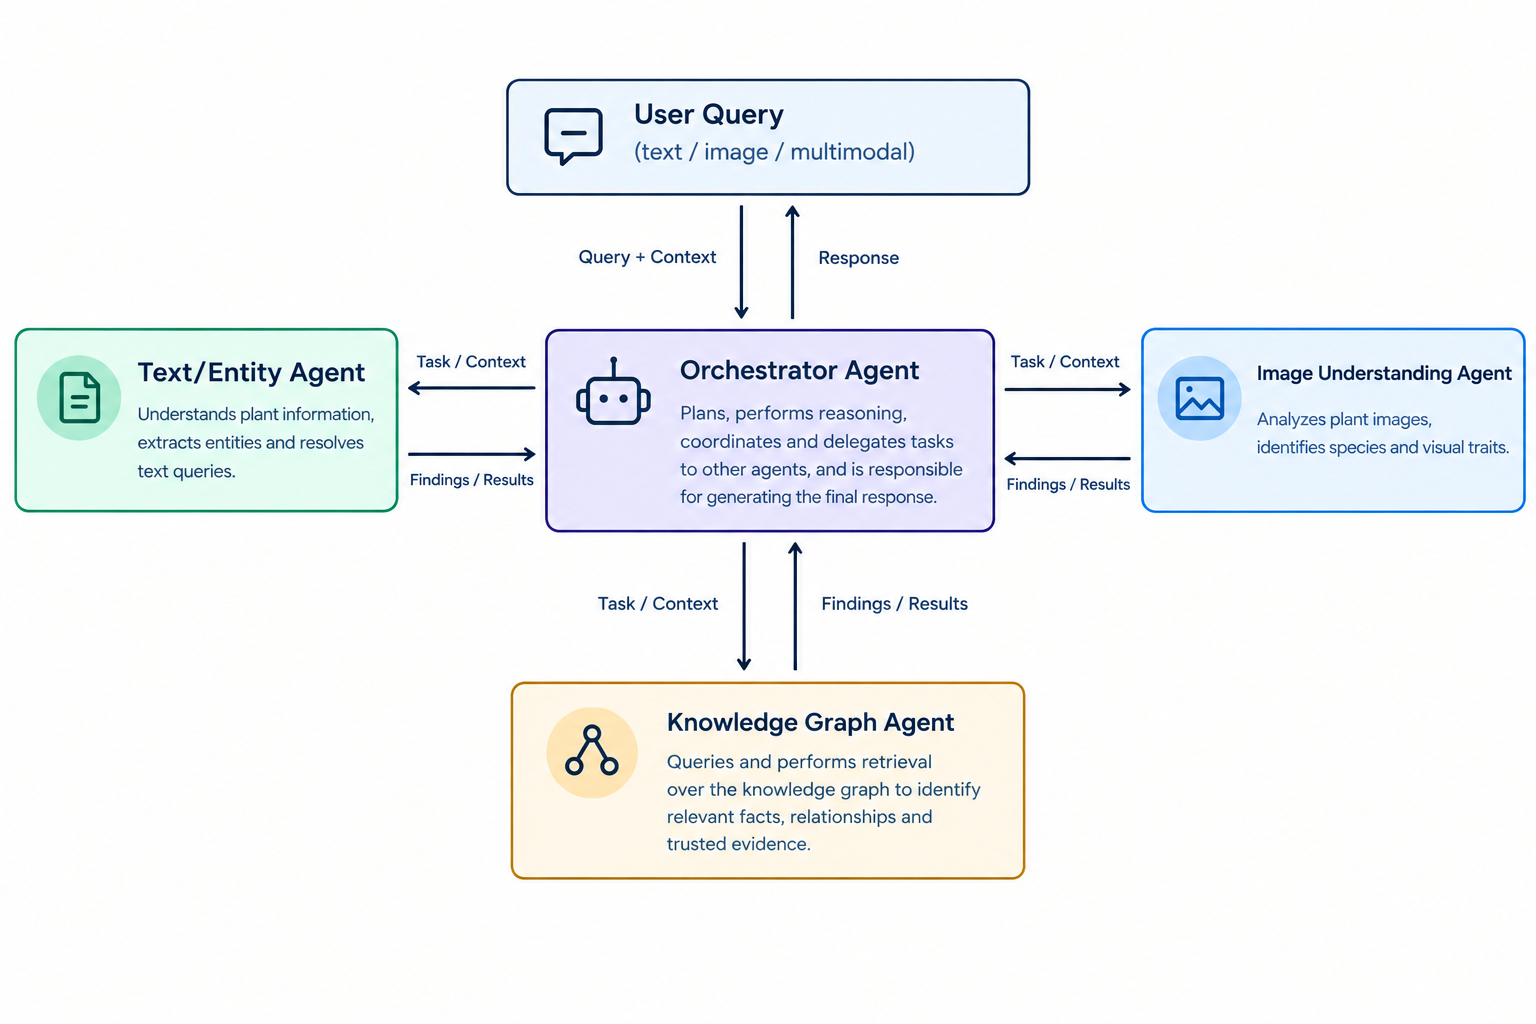
\includegraphics[width=0.98\textwidth]{figures/Multimodal_Agent_Orchestration_Flow.png}
    \caption{Multimodal Agent Orchestration Flow of the proposed platform.}
    \label{fig:overall_flow}
\end{figure}

\subsection{Botanical Discovery and Taxon Resolution Flow}

Every user interaction begins in discovery mode to establish a single verified botanical identity before exploring ethnopharmacological records. Figure~\ref{fig:discovery_seq} depicts the discovery sequence execution.

\begin{figure}[htbp]
    \centering
    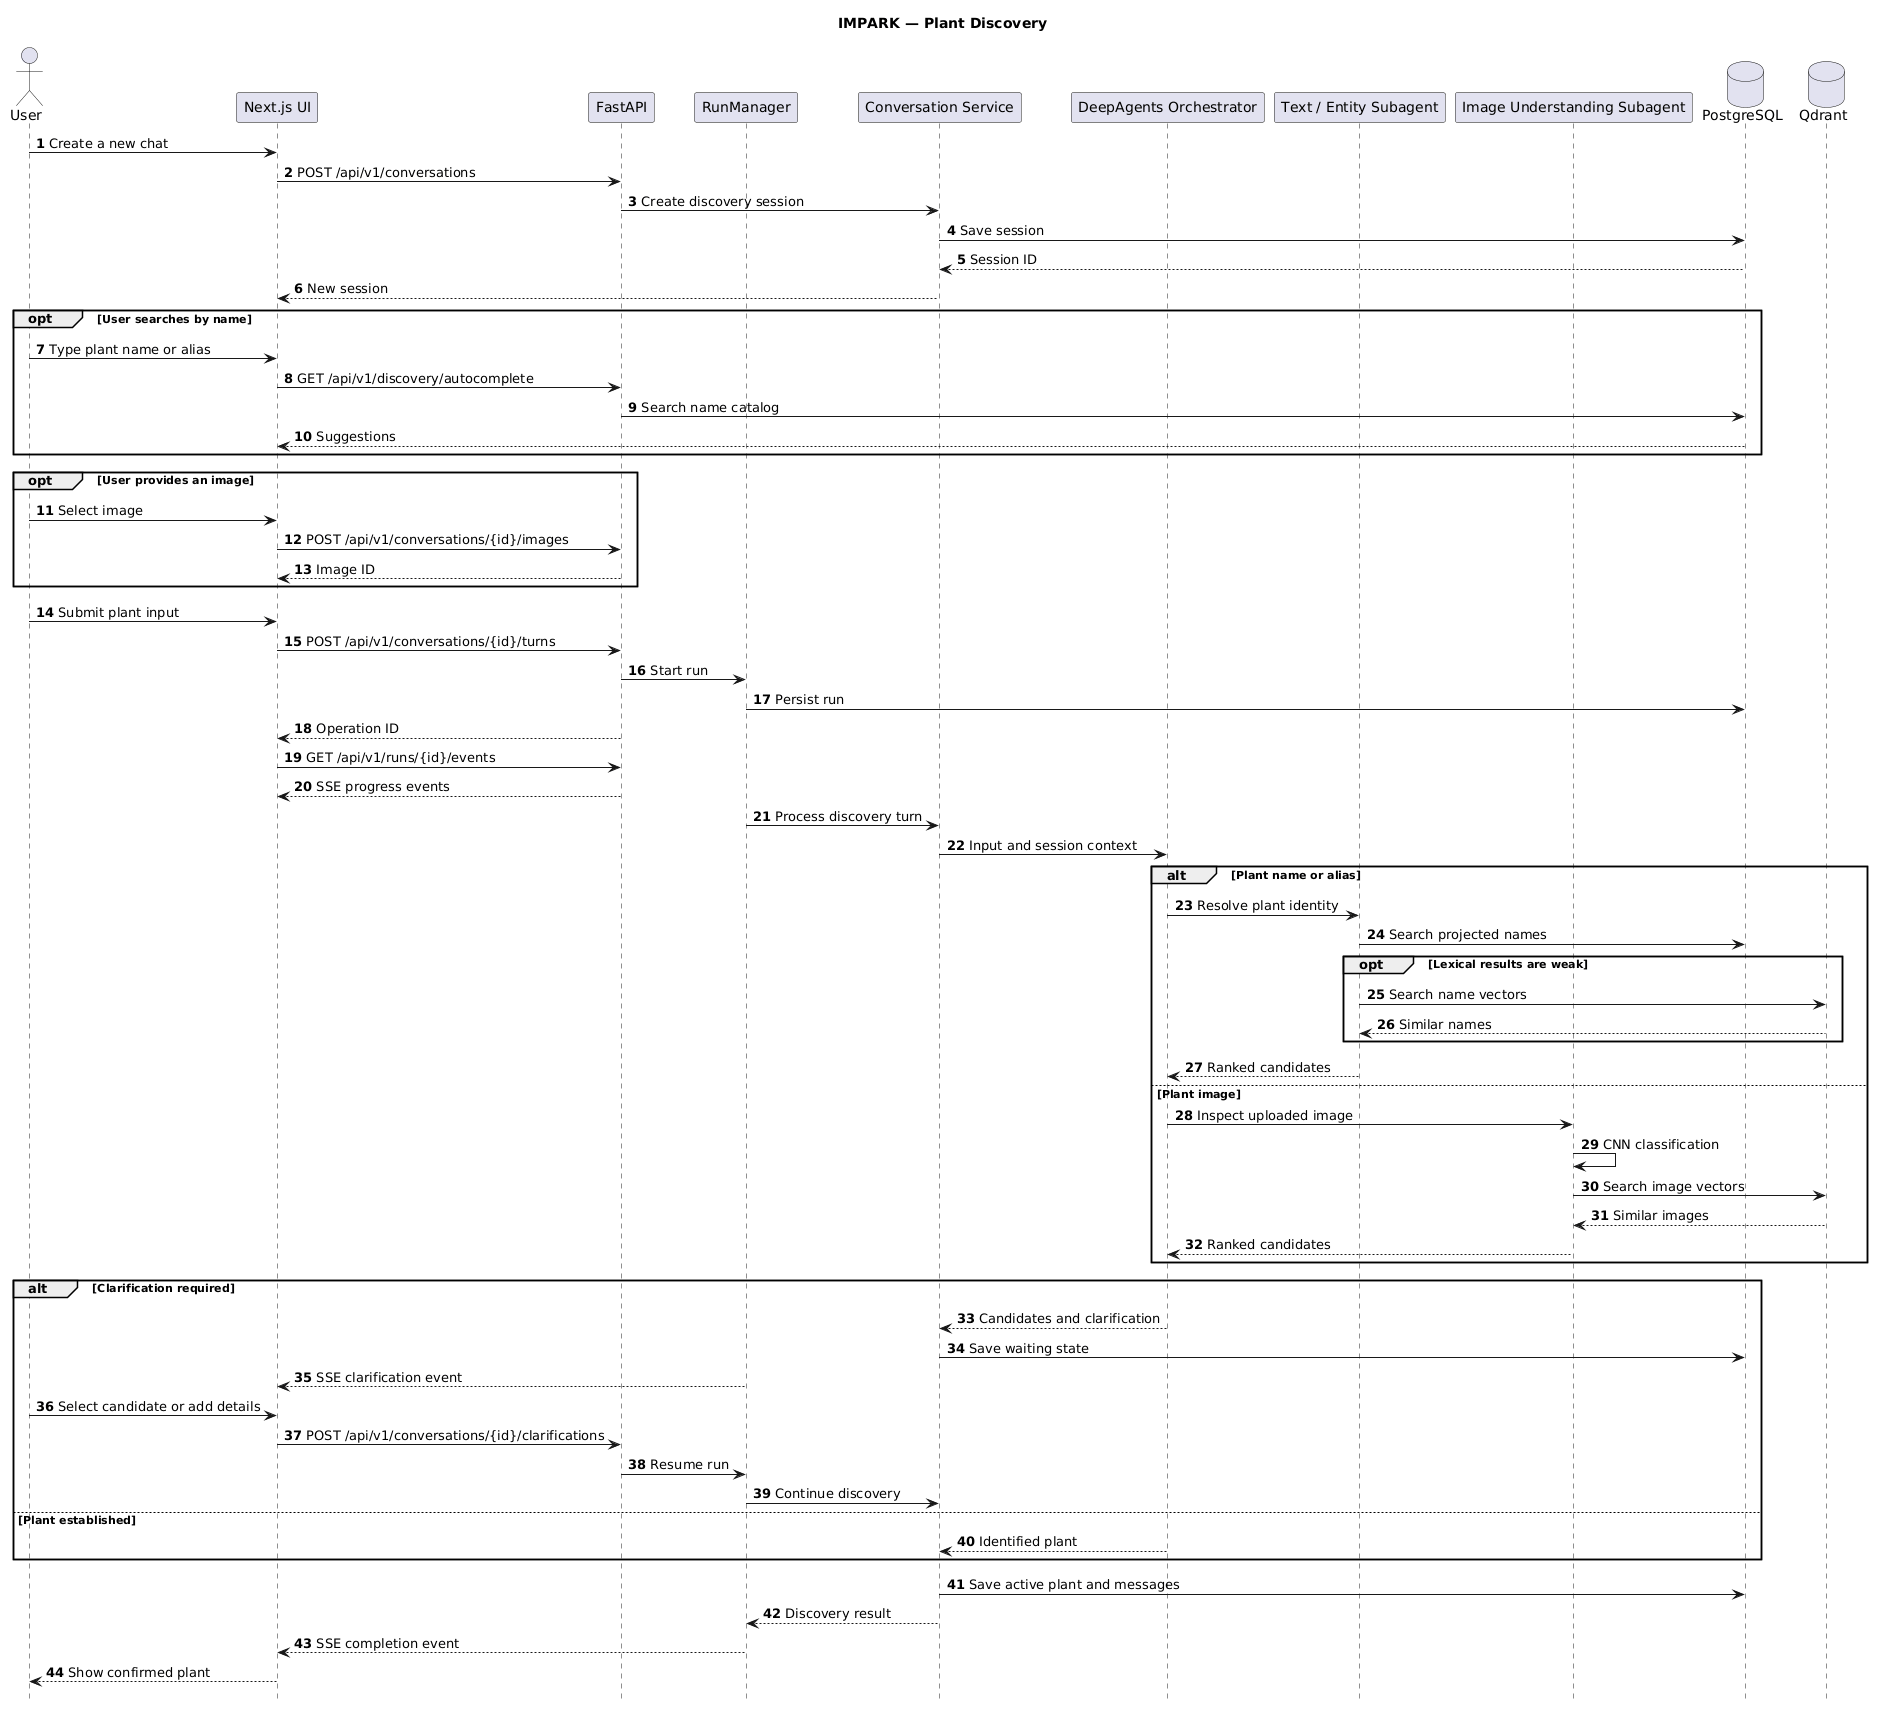
\includegraphics[width=0.88\textwidth]{figures/discovey_phase_sequence_diagram.png}
    \caption{Sequence execution flow during the botanical discovery and identification phase.}
    \label{fig:discovery_seq}
\end{figure}

\begin{enumerate}
    \item \textbf{User Ingestion:} The user submits either a leaf photograph or natural language text specifying common names, medicinal properties, or botanical symptoms.
    \item \textbf{Multimodal Subagent Analysis:}
    \begin{itemize}
        \item When visual input is provided, the Image Understanding Agent computes CNN class probabilities and extracts feature vectors for Qdrant nearest-neighbor retrieval.
        \item When textual input is provided, the Text/Entity Agent applies exact catalog matching, trigram lexical scoring, and multilingual vector search.
    \end{itemize}
    \item \textbf{Candidate Assessment and Locking:} If a candidate taxon achieves dominant confidence ($\ge 0.85$) or leads by a margin $> 0.20$, the plant is automatically locked. If ambiguity exists, the LangGraph outer state machine triggers an \texttt{interrupt()}, emitting a \texttt{clarification\_requested} event to present candidates to the user.
\end{enumerate}

\subsection{Plant-Locked Conversation and Evidence Retrieval Flow}

Once a botanical taxon is confirmed, the conversation locks that plant. Figure~\ref{fig:conversation_seq} illustrates the evidence retrieval flow.

\begin{figure}[htbp]
    \centering
    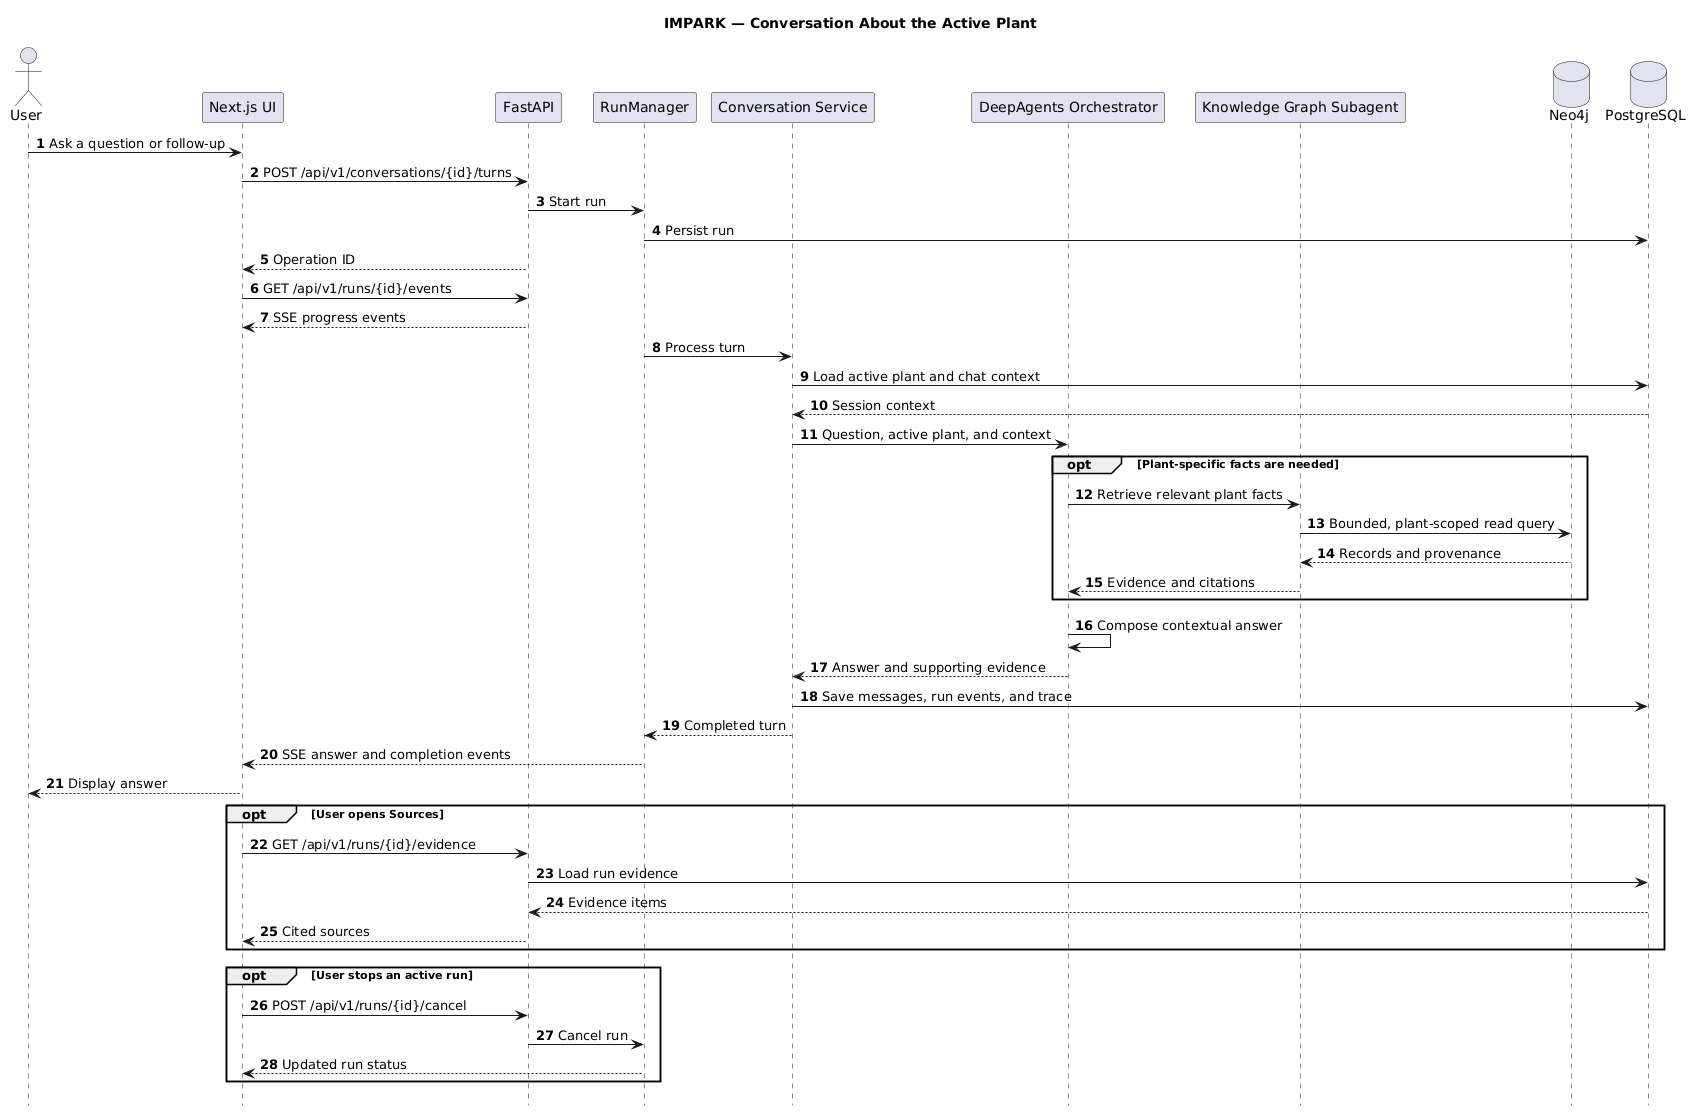
\includegraphics[width=0.92\textwidth]{figures/conversation_phase_sequence_diagram.png}
    \caption{Sequence execution flow during the plant-locked conversation and evidence retrieval phase.}
    \label{fig:conversation_seq}
\end{figure}

During this phase, user inquiries are evaluated against the locked plant context. The coordinator delegates factual queries to the Knowledge Graph Agent, which executes allow-listed Cypher queries over Neo4j, converts paths into structured \texttt{Evidence} blocks, and streams responses with citation badges to the client.

% ============================================================================
% 3.4 Detailed Formulation With Equations
% ============================================================================
\section{Explanation of Methodology in Detail With Equations and Formulae}

\subsection{Overall System Architecture}

The system architecture of the framework, illustrated in Figure~\ref{fig:system_arch}, enforces complete decoupling between the presentation tier, API orchestration gateway, machine learning inference backends, and storage engines.

\begin{figure}[htbp]
    \centering
    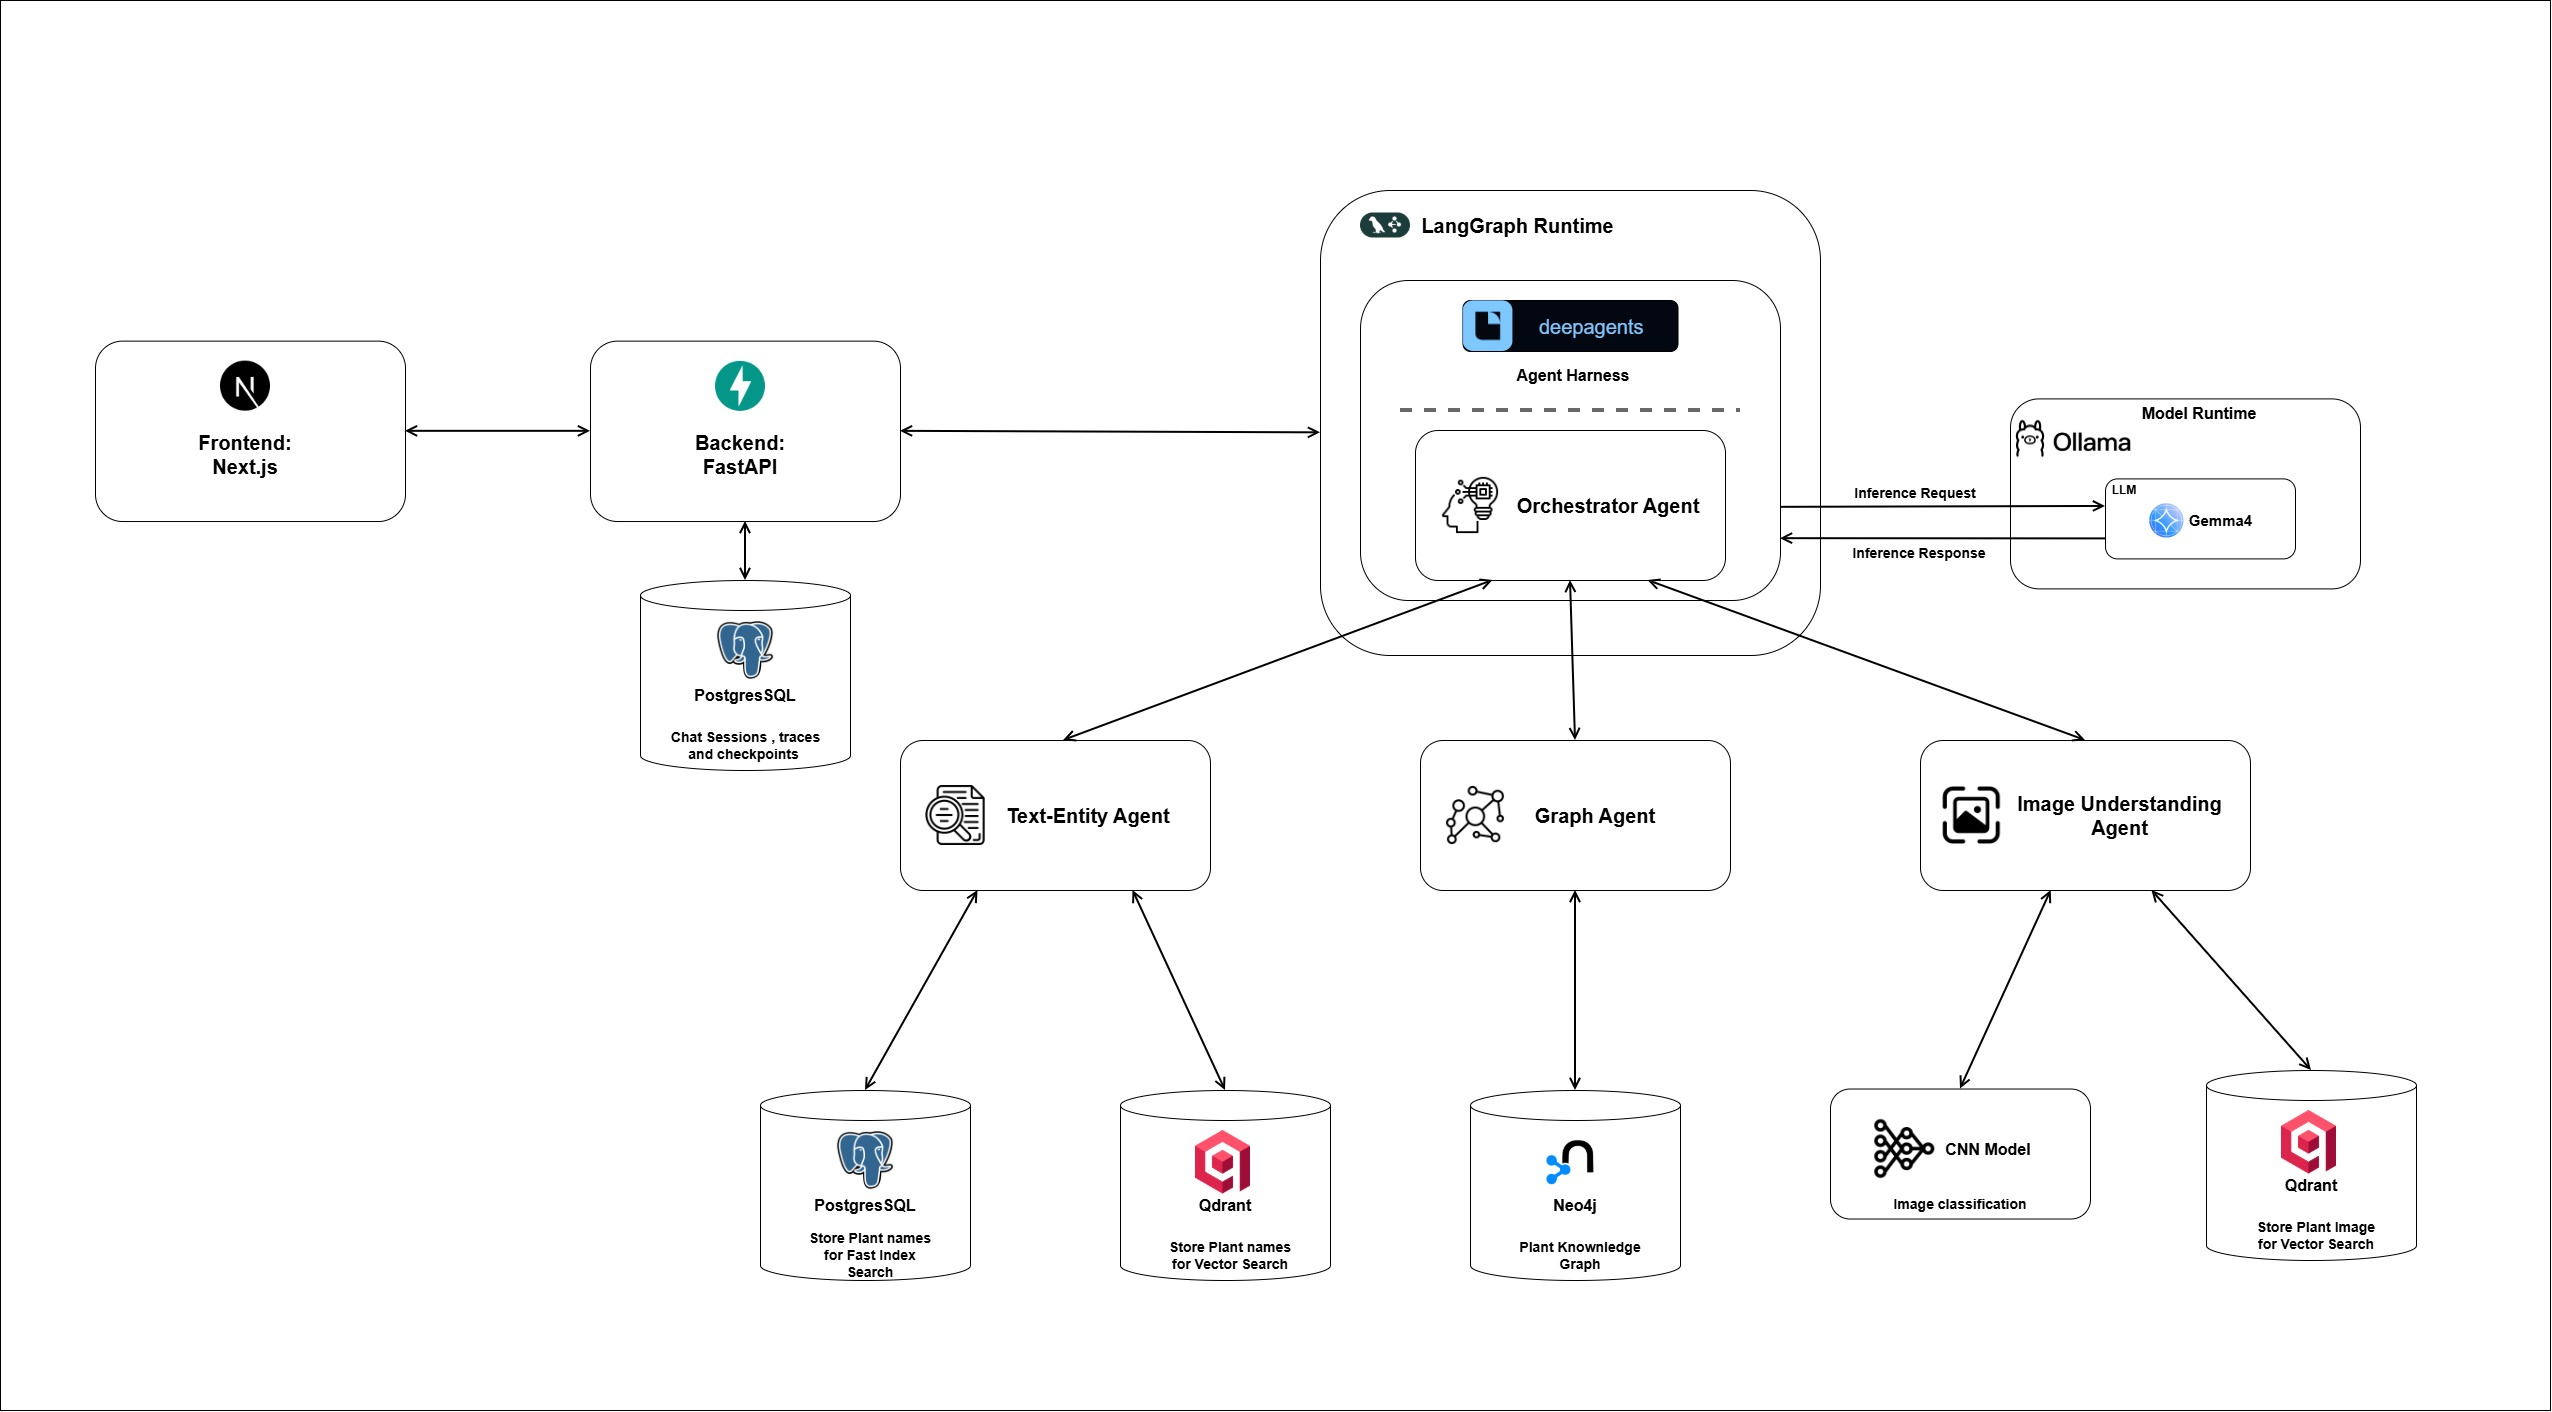
\includegraphics[width=0.92\textwidth]{figures/multiagent-architecture-diagram.jpg}
    \caption{Overall multi-agent system architecture of the proposed platform.}
    \label{fig:system_arch}
\end{figure}

\subsection{Medicinal Plant Leaf Classification and Feature Extraction}

Visual plant identification utilizes a deep convolutional neural network based on the Xception architecture (\texttt{training/\allowbreak image/\allowbreak train\_model.py} and \texttt{backend/\allowbreak agents/\allowbreak image/\allowbreak model.py}), detailed in Figure~\ref{fig:image_agent}.

\begin{figure}[htbp]
    \centering
    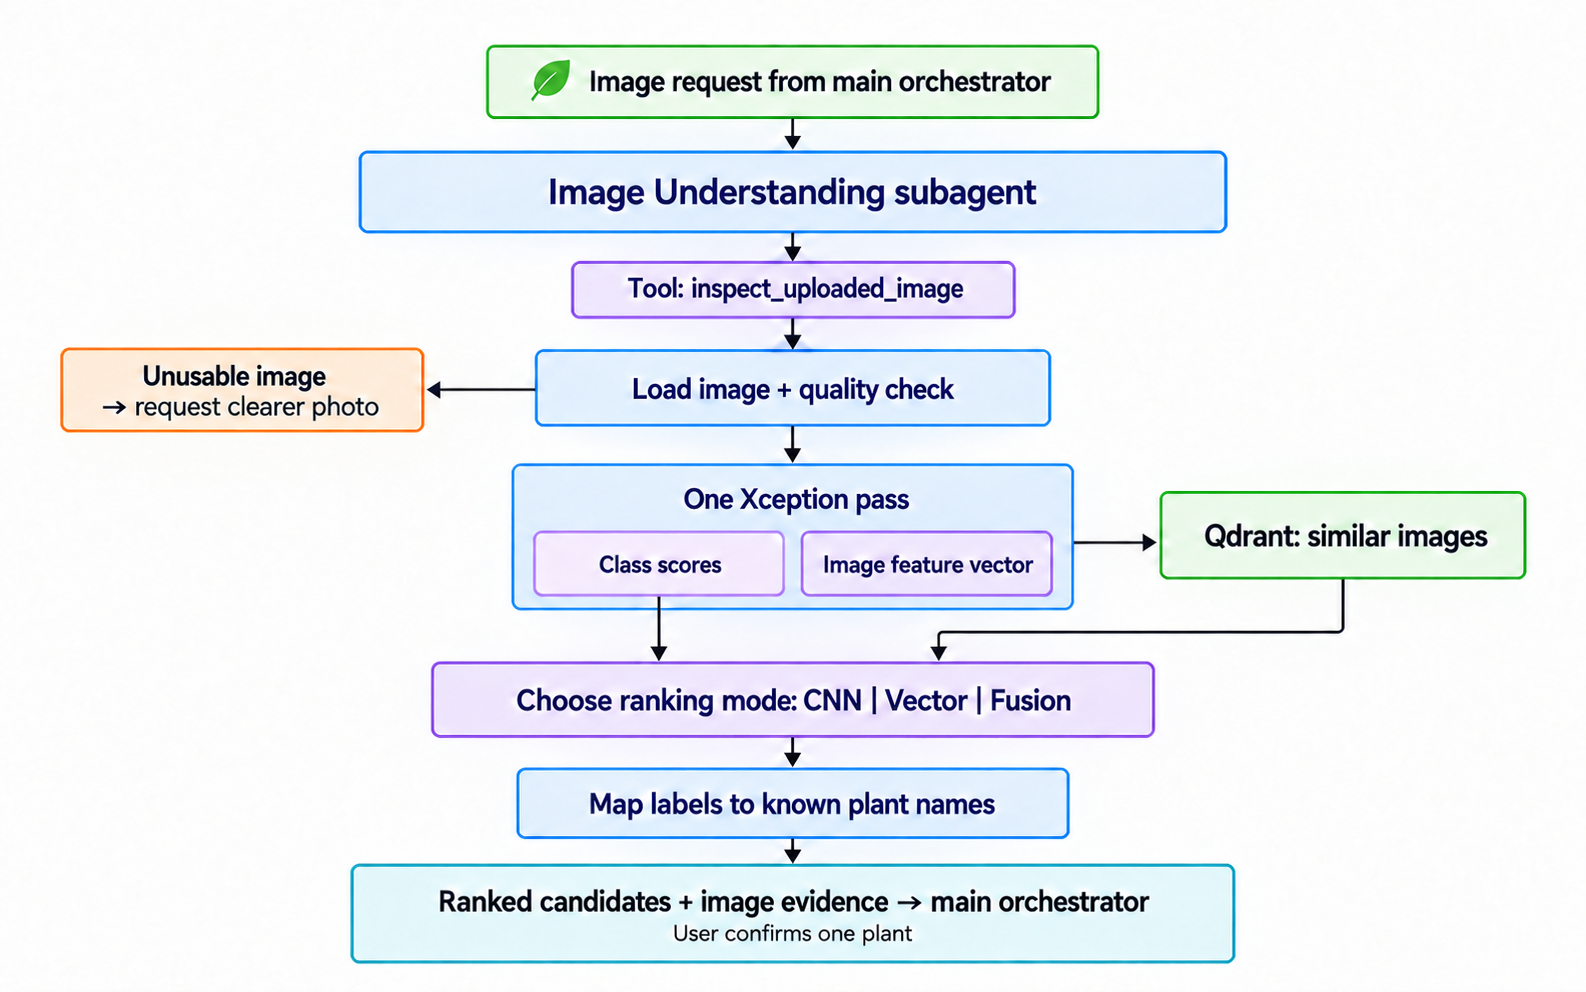
\includegraphics[width=0.95\textwidth]{figures/image-agent-current.png}
    \caption{Image Understanding Agent architecture combining Xception CNN classification and Qdrant vector retrieval.}
    \label{fig:image_agent}
\end{figure}

The network takes a preprocessed RGB image tensor $\mathbf{X} \in \mathbb{R}^{300 \times 400 \times 3}$ and passes it through depthwise separable convolutional blocks. The spatial feature map output by the final convolutional layer is denoted as $\mathbf{A} \in \mathbb{R}^{H \times W \times D}$, where $D = 2,048$. Global Average Pooling computes a 2,048-dimensional feature vector $\mathbf{z} \in \mathbb{R}^{2048}$:
\begin{equation}
z_k = \frac{1}{H \times W} \sum_{i=1}^H \sum_{j=1}^W A_{i,j,k}, \quad k \in \{1, 2, \ldots, 2048\}.
\label{eq:gap}
\end{equation}
Vector $\mathbf{z}$ is processed through Batch Normalization and passed into a fully connected layer with weight matrix $\mathbf{W}_1 \in \mathbb{R}^{256 \times 2048}$ and bias vector $\mathbf{b}_1 \in \mathbb{R}^{256}$:
\begin{equation}
\mathbf{h} = \operatorname{ReLU}(\mathbf{W}_1 \mathbf{z} + \mathbf{b}_1).
\label{eq:dense_relu}
\end{equation}
After applying dropout ($p = 0.40$), the intermediate representation is mapped to class logits $\mathbf{o} = \mathbf{W}_2 \mathbf{h} + \mathbf{b}_2 \in \mathbb{R}^{40}$. The Softmax function computes posterior class probabilities:
\begin{equation}
P_{\mathrm{CNN}}(y = c \mid \mathbf{X}) = \frac{\exp(o_c)}{\sum_{j=1}^{40} \exp(o_j)}, \quad c \in \{1, 2, \ldots, 40\}.
\label{eq:softmax}
\end{equation}
Simultaneously, pooled feature vector $\mathbf{z}$ is normalized to unit $L_2$ length to serve as visual retrieval query vector $\mathbf{v}$:
\begin{equation}
\mathbf{v} = \frac{\mathbf{z}}{\|\mathbf{z}\|_2} = \frac{\mathbf{z}}{\sqrt{\sum_{k=1}^{2048} z_k^2}}.
\label{eq:l2_norm}
\end{equation}

\subsection{Auditable Nearest-Neighbor Retrieval and Hybrid Score Fusion}

Visual query vector $\mathbf{v}$ is queried against the \texttt{plant\_images\_v1} collection in Qdrant using cosine similarity:
\begin{equation}
S_{\mathrm{visual}}(\mathbf{v}, \mathbf{u}_i) = \frac{\mathbf{v} \cdot \mathbf{u}_i}{\|\mathbf{v}\|_2 \|\mathbf{u}_i\|_2} = \sum_{k=1}^{2048} v_k u_{i,k}.
\label{eq:cosine_sim}
\end{equation}
For each candidate taxon label $l$, the $k$-NN visual score $P_{\mathrm{kNN}}(y = l \mid \mathbf{X})$ is computed from the top-$K$ nearest neighbors ($K = 5$):
\begin{equation}
P_{\mathrm{kNN}}(y = l \mid \mathbf{X}) = \frac{\sum_{i \in \mathcal{N}_K, \, \mathrm{label}(i) = l} S_{\mathrm{visual}}(\mathbf{v}, \mathbf{u}_i)}{\sum_{i \in \mathcal{N}_K} S_{\mathrm{visual}}(\mathbf{v}, \mathbf{u}_i)}.
\label{eq:knn_score}
\end{equation}
The final hybrid visual confidence score $S_{\mathrm{image}}(l)$ is computed via convex combination with weight $\alpha = 0.65$:
\begin{equation}
S_{\mathrm{image}}(l) = \alpha \cdot P_{\mathrm{CNN}}(y = l \mid \mathbf{X}) + (1 - \alpha) \cdot P_{\mathrm{kNN}}(y = l \mid \mathbf{X}).
\label{eq:hybrid_image}
\end{equation}

\subsection{Cascaded Hybrid Entity Search and RapidFuzz Scoring}

Natural language queries are evaluated through the three-tier resolution pipeline depicted in Figure~\ref{fig:text_agent}.

\begin{figure}[htbp]
    \centering
    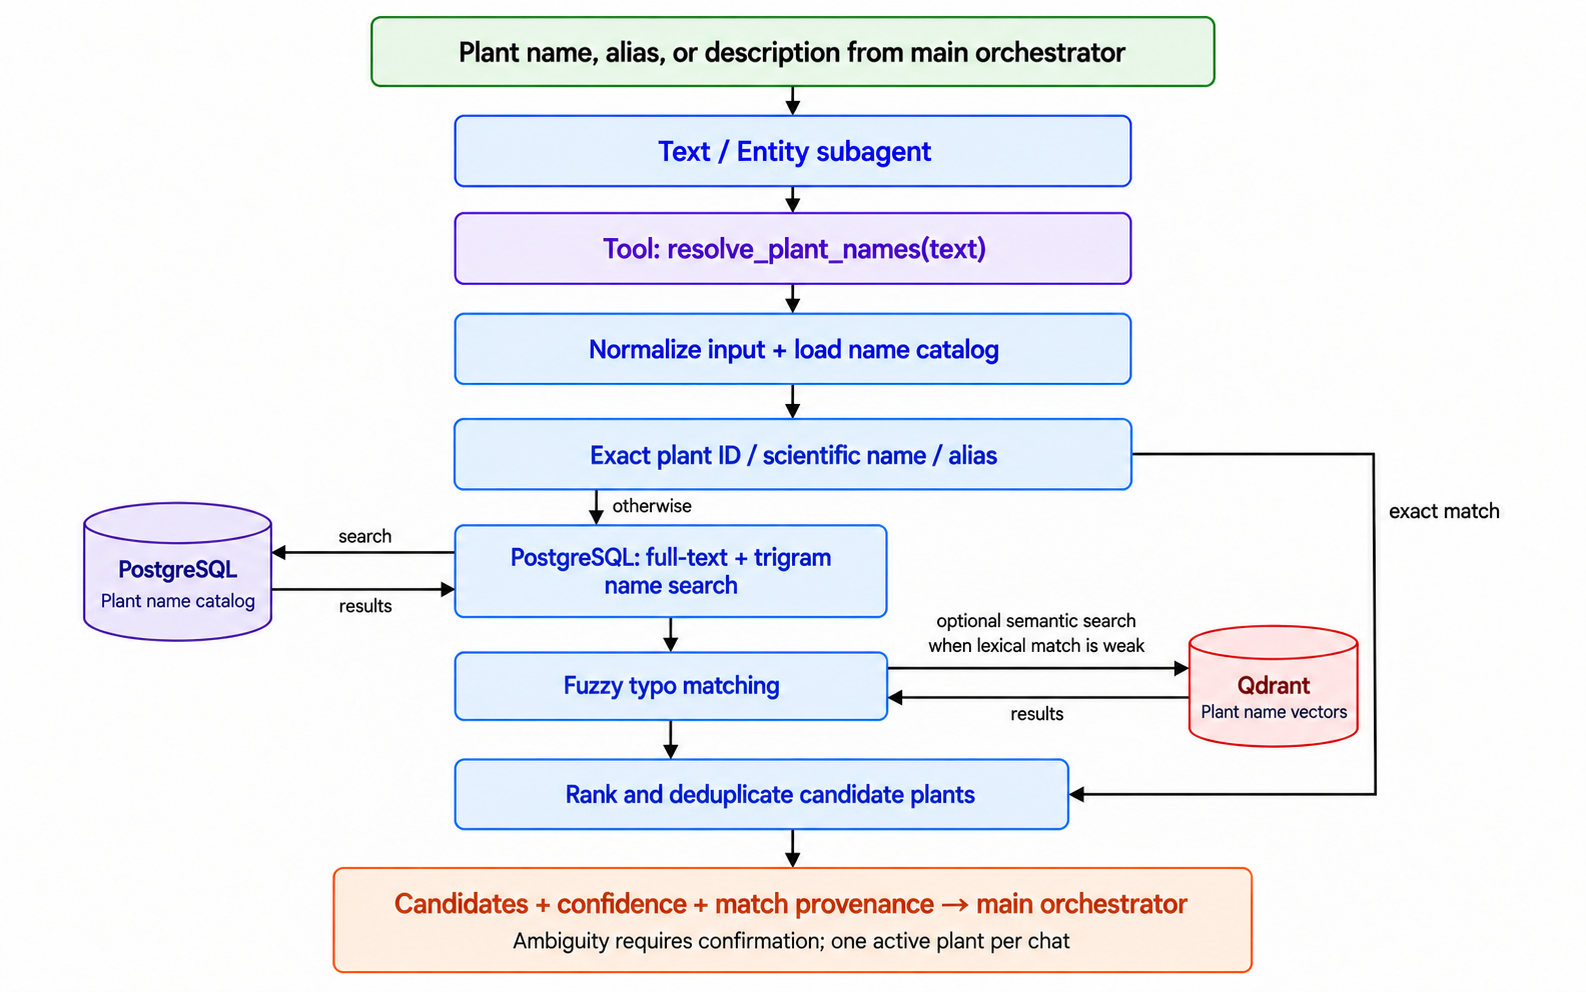
\includegraphics[width=0.95\textwidth]{figures/text-entity-agent-current.png}
    \caption{Text and Entity Agent resolution pipeline incorporating exact catalog lookup, trigram matching, and multilingual vector search.}
    \label{fig:text_agent}
\end{figure}

The resolution process cascades through three stages:
\begin{enumerate}
    \item \textbf{Exact Match:} Evaluates normalized query string $q$ against pre-indexed alias records in PostgreSQL:
    \begin{equation}
    S_{\mathrm{exact}}(c) = \mathbb{I}(q \in \mathcal{A}_c), \quad S_{\mathrm{exact}} \in \{0, 1\}.
    \end{equation}
    \item \textbf{Fuzzy Lexical Matching:} Computes character trigram similarity and token-sort ratios using RapidFuzz:
    \begin{equation}
    S_{\mathrm{fuzzy}}(c) = \max_{a \in \mathcal{A}_c} \frac{2 \cdot |T(q) \cap T(a)|}{|T(q)| + |T(a)|} \in [0, 1].
    \label{eq:trigram_dice}
    \end{equation}
    \item \textbf{Dense Semantic Search:} Queries text embeddings using FastEmbed ($d = 384$):
    \begin{equation}
    S_{\mathrm{semantic}}(c) = \max_{d \in \mathcal{D}_c} \cos(\phi(q), \phi(d)).
    \label{eq:semantic_sim}
    \end{equation}
\end{enumerate}
Reciprocal Rank Fusion (RRF) combines lexical and semantic search rankings into unified confidence score $S_{\mathrm{text}}(c)$:
\begin{equation}
S_{\mathrm{text}}(c) = \frac{1}{60 + R_{\mathrm{fuzzy}}(c)} + \frac{1}{60 + R_{\mathrm{semantic}}(c)}.
\label{eq:rrf}
\end{equation}

\subsection{Knowledge Graph Schema and Parameterized Cypher Retrieval}

Figure~\ref{fig:graph_schema} illustrates the Neo4j ontological schema, and Figure~\ref{fig:graph_agent} depicts the Knowledge Graph Agent query pipeline.

\begin{figure}[htbp]
    \centering
    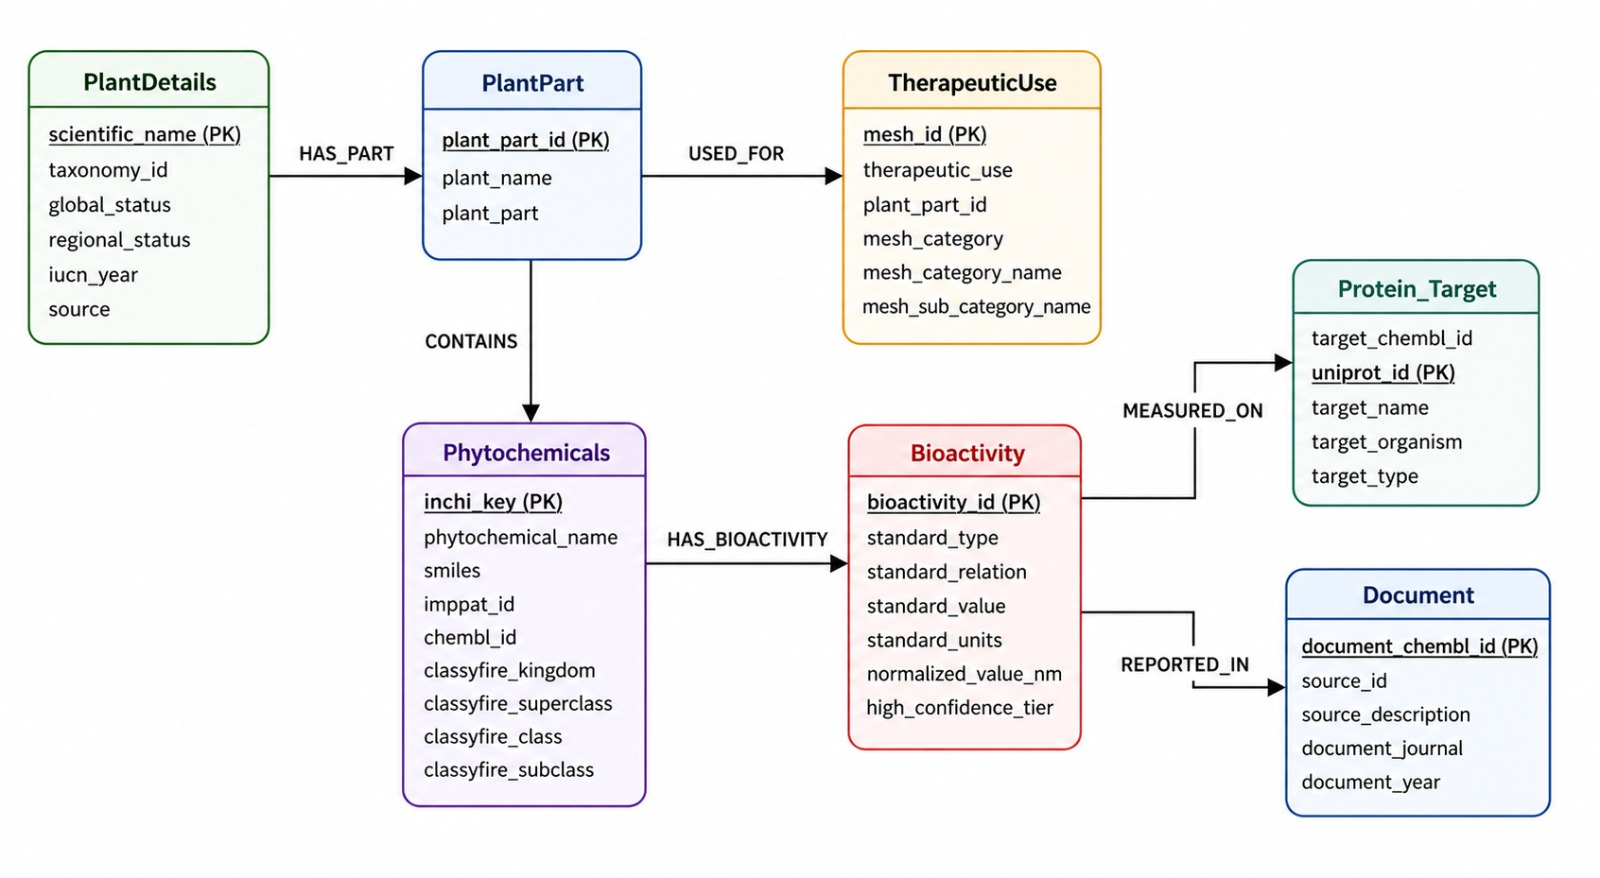
\includegraphics[width=0.88\textwidth]{figures/new_schema.jpeg}
    \caption{Neo4j Knowledge Graph ontological schema and relationship topology.}
    \label{fig:graph_schema}
\end{figure}

\begin{figure}[htbp]
    \centering
    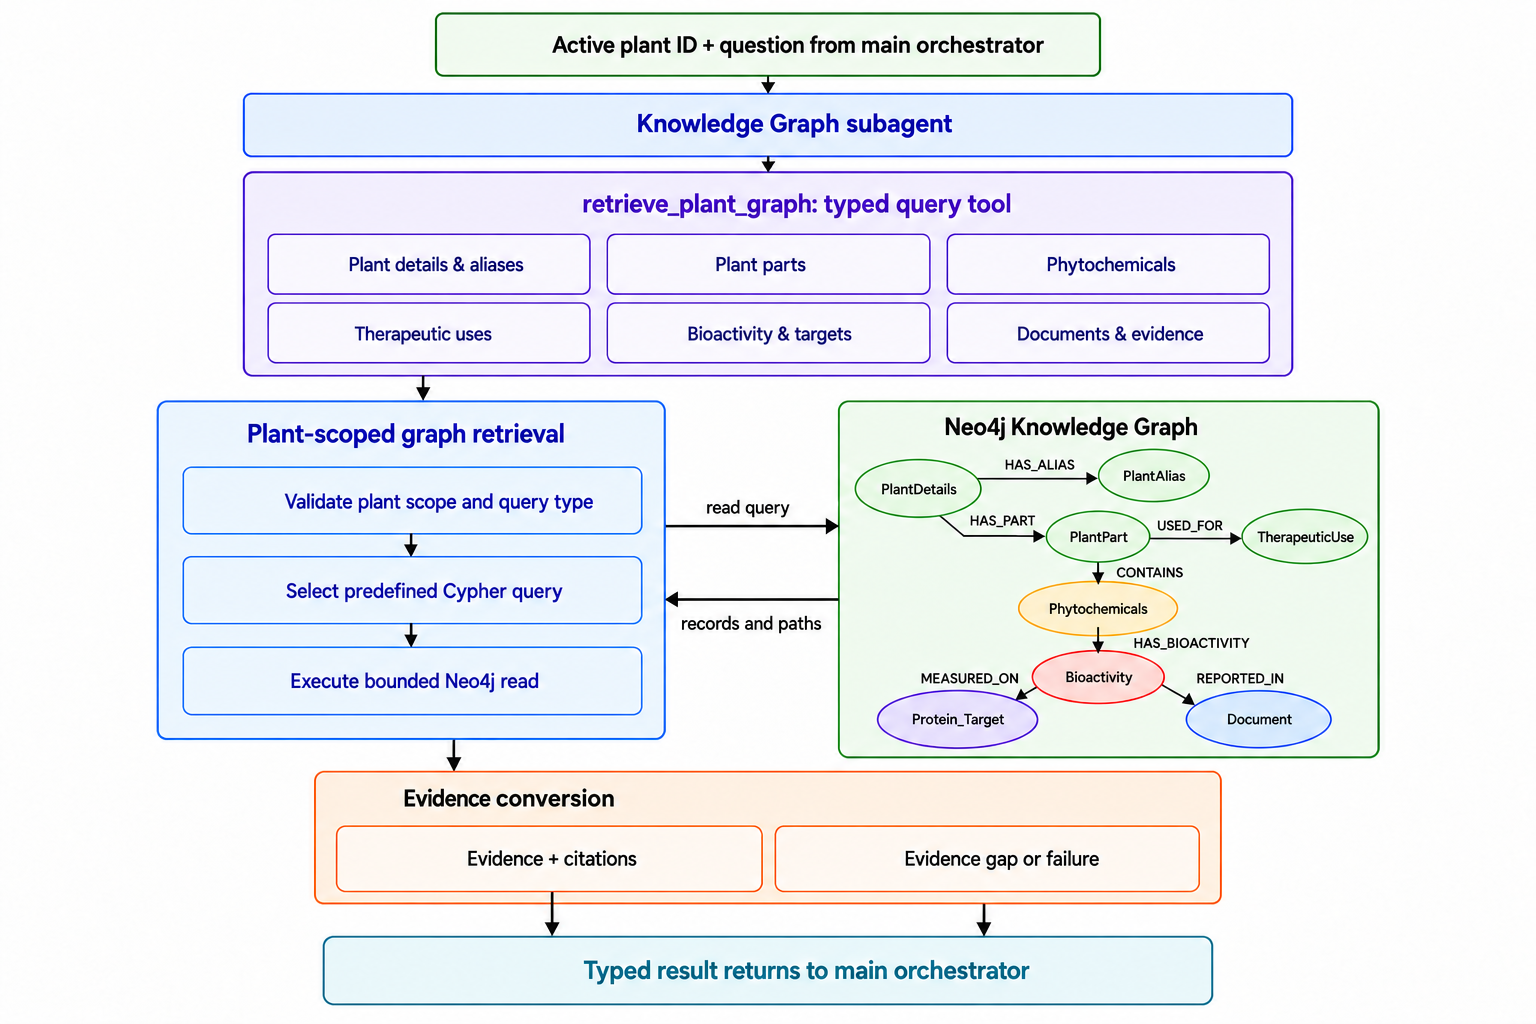
\includegraphics[width=0.95\textwidth]{figures/graph-agent-current.png}
    \caption{Knowledge Graph Agent retrieval architecture with parameterized Cypher templates and evidence packaging.}
    \label{fig:graph_agent}
\end{figure}

The \texttt{retrieve\_plant\_graph} tool delegates requests to parameterized Cypher templates. Representative query templates include:
\begin{equation}
\mathcal{Q}_{\mathrm{safe}}(p, \mathcal{C}) = \mathtt{MATCH}\;(p\mathtt{:PlantDetails})\mathtt{-}[r]\mathtt{-}(n)\;\mathtt{WHERE}\;p.\mathrm{plant\_name} = \$name\;\mathtt{RETURN}\;p, r, n.
\label{eq:cypher_template}
\end{equation}
Each retrieved record is transformed into an immutable \texttt{Evidence} object. The object encapsulates the factual JSON payload, graph relationship sequence, traversed node representations, external reference URLs, and a deterministic UUID version 5 identifier:
\begin{equation}
\mathrm{ID}_{\mathrm{evidence}} = \mathrm{UUIDv5}\Big(\mathrm{NAMESPACE\_URL},\, \mathrm{str}(\mathrm{ID}_{\mathrm{plant}}) + \operatorname{serialize}(\mathrm{record})\Big).
\label{eq:uuid_evidence}
\end{equation}

\subsection{Dialogue Checkpointing, Disambiguation Interruption, and SSE Streaming}

The outer LangGraph state machine manages session resumption and human-in-the-loop disambiguation. Let the global dialogue state at turn $t$ be denoted as $S_t = \langle M_t, \mathrm{ID}_{\mathrm{plant}}, C_t, E_t \rangle$. When entity resolution is ambiguous ($s_{\max} < 0.60$ or score margin $\Delta < 0.20$), the state machine executes an interruption:
\begin{equation}
S_{t+1} = \operatorname{interrupt}\Big(\mathcal{K}_{\mathrm{candidates}},\, \text{"Ambiguous botanical identity"}\Big).
\label{eq:interrupt}
\end{equation}
The entire dialogue state is serialized into PostgreSQL via \texttt{AsyncPostgresSaver}. Once the user confirms the intended taxon, execution resumes along the checkpoint lineage. Post-generation processing enforces scientific compliance (\texttt{backend/\allowbreak orchestrator/\allowbreak deepagents/\allowbreak response\_quality.py}), ensuring that species-specific claims are grounded in retrieved graph evidence before streaming tokens to the client over Server-Sent Events.
